

\section{Zero- and Few-Shot Inference}
Prompting methods can often be used without \emph{any} explicit training of the language model (LM) for the downstream task. One can take an LM that has been trained to predict the probability of text $P(\bm{x})$ and apply it as-is to fill the cloze or prefix prompts that define the task. This is traditionally referred to as the \emph{zero-shot} setting, as there is no training data available for the task of interest.

However, in the scenario where a limited number of labeled examples are available or can be easily annotated, it is possible to augment the prompt to include this additional information. This setting is referred to as \emph{few-shot} inference and consists of including a small collection of input-out exemplars. These exemplars are input-output pairs that serve as demonstrations of the behavior that one would like the LM to emulate. By using these pairs as a guide, the large LMs can learn to carry out the desired task. This simple idea was shown to
for example, we can augment the standard prompt ``France’s capital is \texttt{[X]} .’’ by prepending a few examples such as ``Great Britain's capital is London . Germany's capital is Berlin . France’s capital is \texttt{[X]}'’. Note that few-shot inference does not involve any parameter updates.

The introduction of GPT-3 \citep{brown2020language} popularized this approach: the model was shown to benefit from the inclusion of exemplars in the prompt on a wide range of tasks and across different model sizes. An example of this behavior is displayed in \Cref{fig:fsl}.

\begin{figure}[ht]
    \centering
    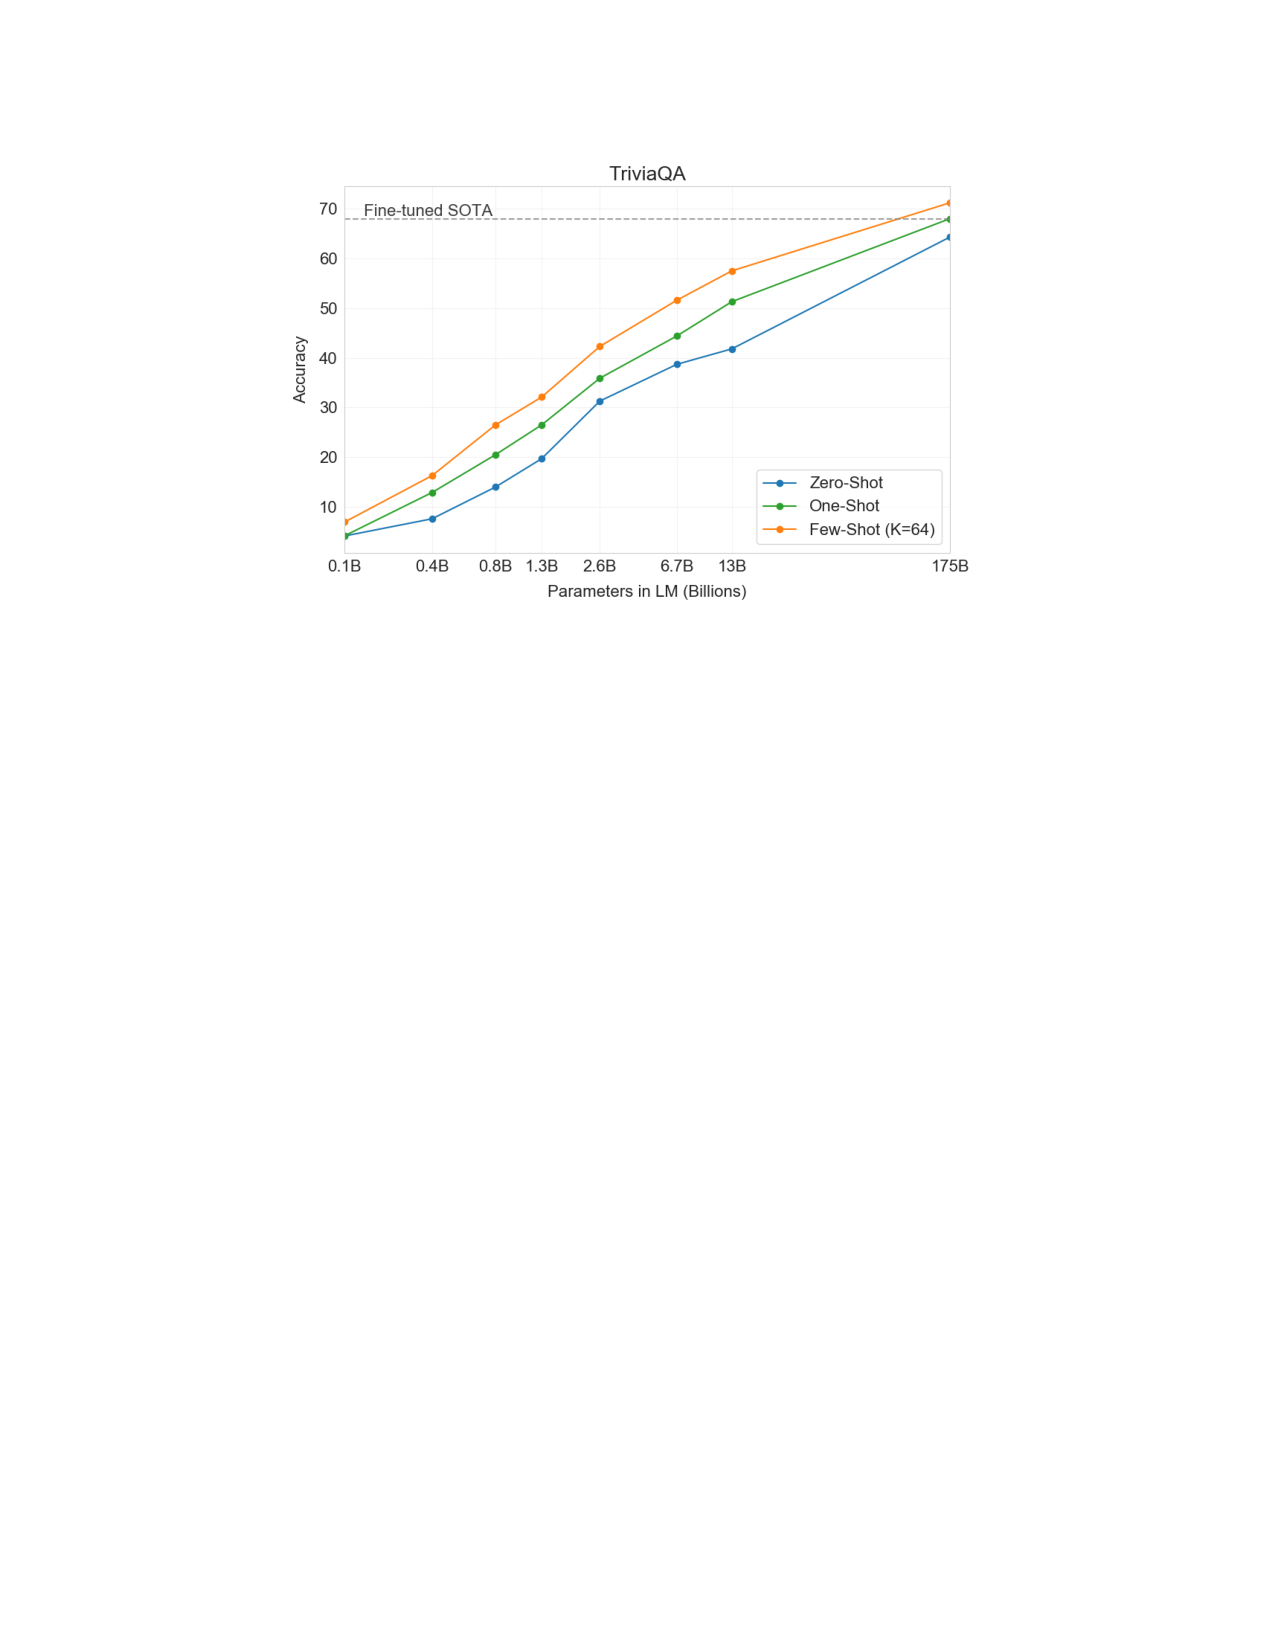
\includegraphics[width=0.8\textwidth]{figures/prompting_and_zero_shot/fsl.pdf}
    \caption{Results of GPT-3 on the TriviaQA dataset, using different numbers of exemplars in the few-shot prompt. From \citet{brown2020language}.
    }
    \label{fig:fsl}
\end{figure}

Although the idea of including a small number of examples in the prompt is simple, there are some aspects that we need to pay attention to: (1) what examples should be included in the prompt to make the demonstration effective, and (2) how to order the examples in the prompt.
Regarding the example selection, researchers have shown that different demonstrations can result in very different performance \citep{lu2021fantastically}. An approach to tackle this issue consists of using sentence embeddings to sample examples that are close to the input in the embedding space \citep{liu-etal-2022-makes, drori2022neural}. As for the order of the labeled examples, methods were proposed to score different candidate permutations \citep{lu2021fantastically}.


\subsection{In-Context Learning}
In-context learning is an \textit{emergent behavior} displayed by large LMs that can lead to the models performing previously unseen tasks in a few-shot setting, without any parameter optimization. 

Initially pointed out by \cite{brown2020language} in the presentation of the GPT-3 model, this behavior has been the subject of several studies and surveys. Notably, the phenomenon occurs suddenly as the model size increases, leading to the definition of emergent behavior. While including a few exemplars in the prompt does not lead to a significant difference in performance in small-scale models, it leads to a significantly improved behavior in large models (e.g., GPT-3, PaLM). Another aspect that makes this behavior surprising is the mismatch between the LM’s training objective and the tasks that the model is able to learn in-context. Typically, large LMs are trained with a self-supervised language modeling objective, and the mechanisms that allow these models to learn a previously unseen task (e.g., text classification) without any parameter optimization are currently an active area of research.

Recent work has hypothesized that in-context learning by few-shot prompting works as a process of meta-optimization on the few examples included in the prompt \citep{dai2022can}. The authors show experimental results that support the idea that, when performing in-context learning, the models produce meta-gradients according to the demonstration exemplars through forward computation. Then these meta gradients are applied to the original LM through attention. This way, in-context learning can be seen as a kind of implicit fine-tuning on the few-shot exemplars.



\section{Popular Prompting Strategies}
In this section, we dive deeper into some of the most popular prompting strategy aimed at eliciting in-context learning in various LLMs.

%\mrinmaya{Key results}

\subsection{Chain of Thought Prompting}
Multiple studies investigating the reasoning capabilities of large LMs, highlighted how eliciting the model to produce a step-by-step solution of a problem can lead to a more accurate final answer \citep{nye2021show}.
Combining this idea with the intuition of including a set of demonstrations in the prompt, \cite{wei2022chain} introduced the concept of chain of thought (CoT) prompting. Given a question, a \emph{chain of thought} is a coherent sequence of reasoning steps that leads to a final answer. One of the intuitions is that by allowing the model to generate a step-by-step solution, we let the model apply computation proportional to the problem difficulty level (more tokens are generated for problems with more steps).
\Cref{fig:cot} shows an example of a math world problem that the model is able to solve through CoT prompting, and that would otherwise be gotten incorrect.
The step-by-step reasoning displayed by LM through this prompting technique was subsequently shown to be elicited in a zero-shot setting \citep{kojima2022large}. This was achieved simply by adding ``Let's think step-by-step'' to the prompt before the model's answer.

\begin{figure}[htbp]
    \centering
    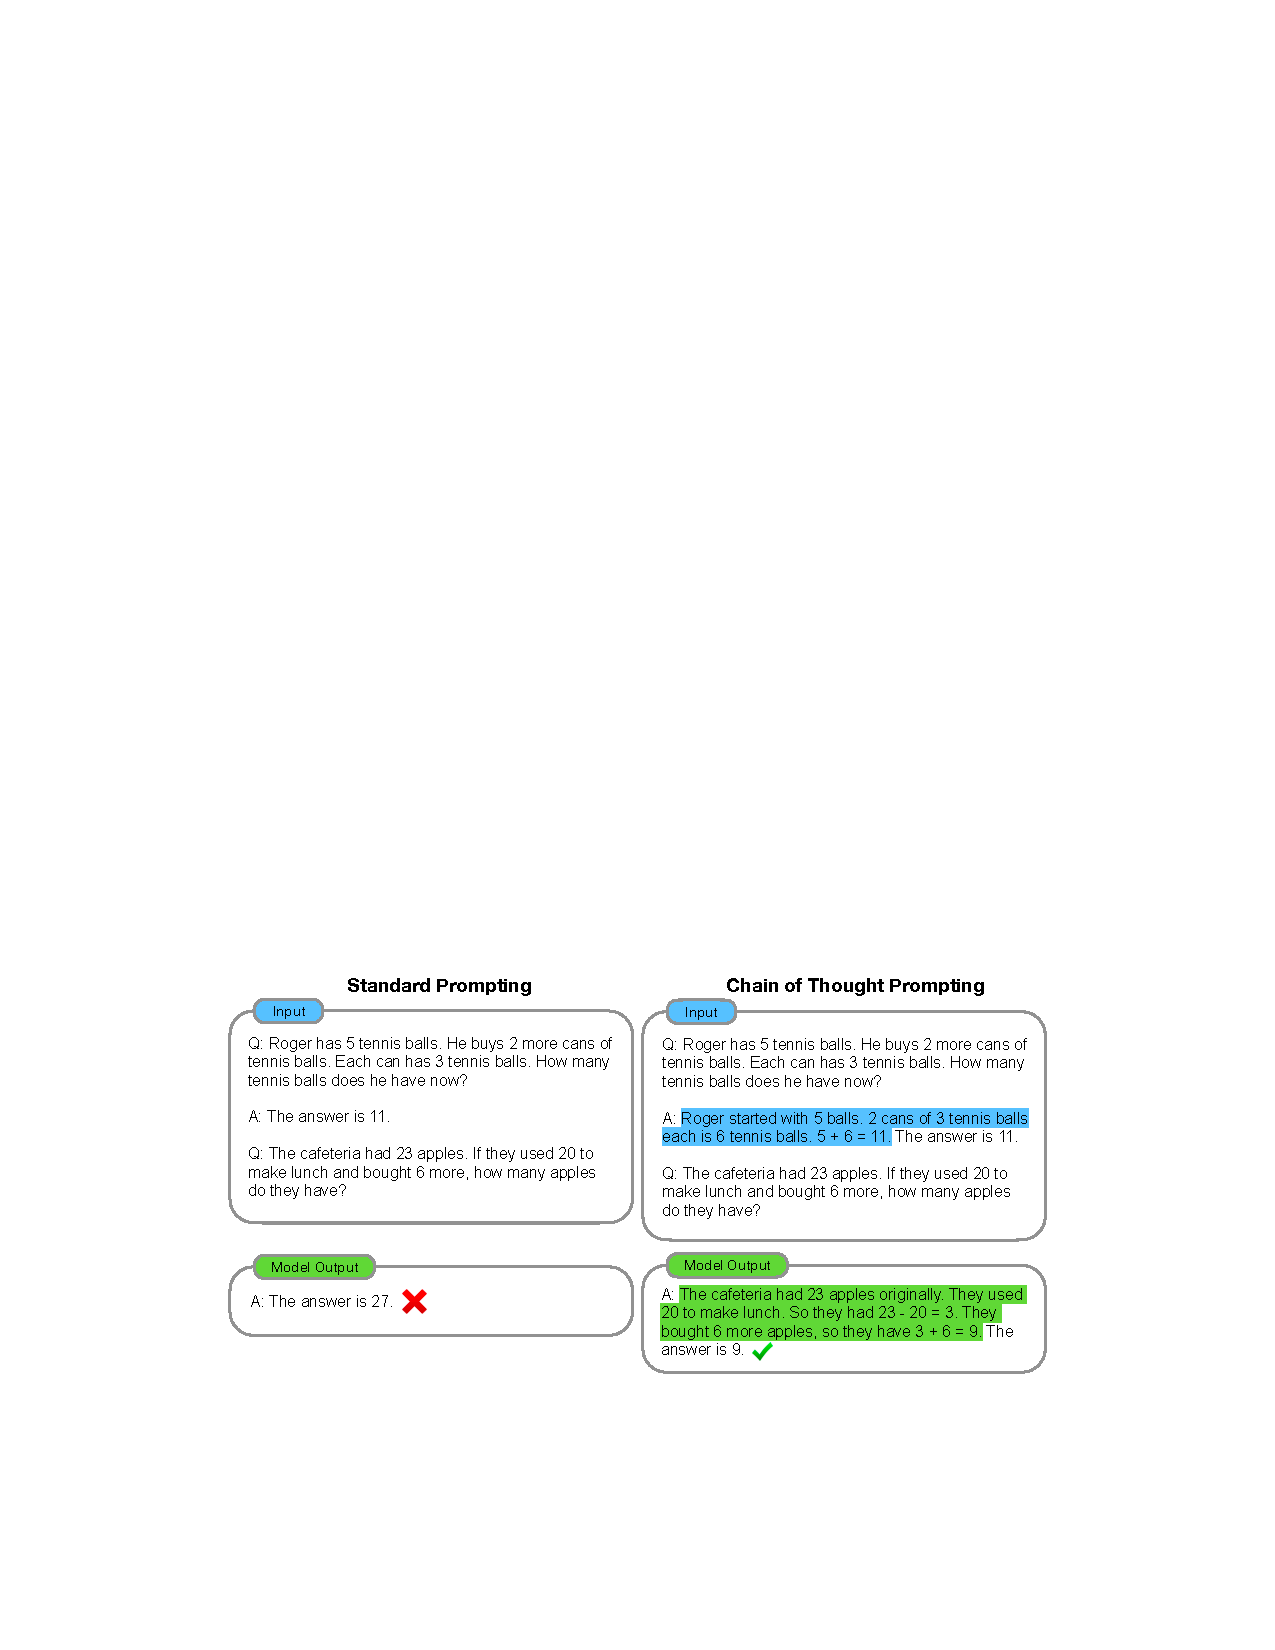
\includegraphics[width=0.9\textwidth]{figures/prompting_and_zero_shot/cot.pdf}
    \caption{Example of the Chain of Thought prompting. Notice the difference between the step-by-step example highlighted in blue and the standard answer only. Taken from \citet{wei2022chain}.
    }
    \label{fig:cot}
\end{figure}

% \begin{figure}[htbp]
%   \centering
%   % Vilém: split legend
%     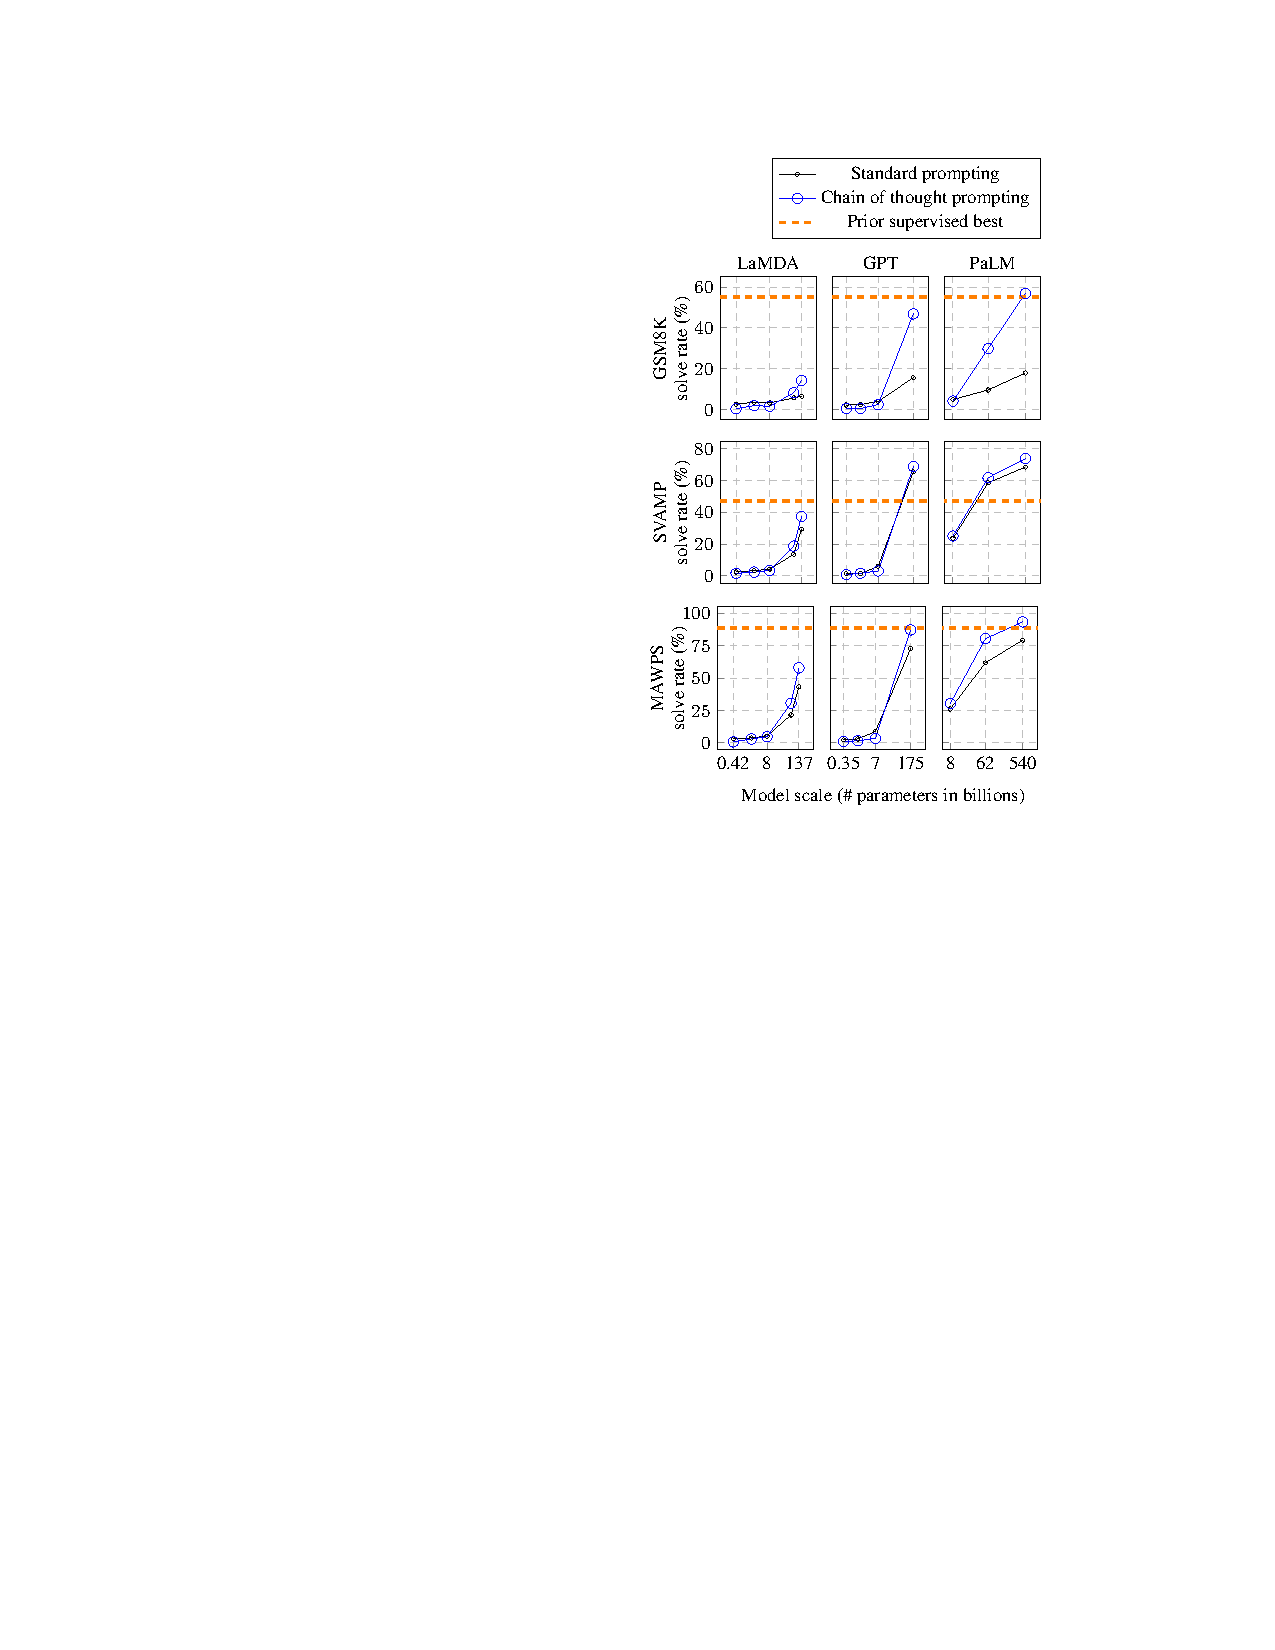
\includegraphics[width=0.4\textwidth,trim={0 0 0 1.6cm},clip]{figures/prompting_and_zero_shot/cot_results.pdf}
%     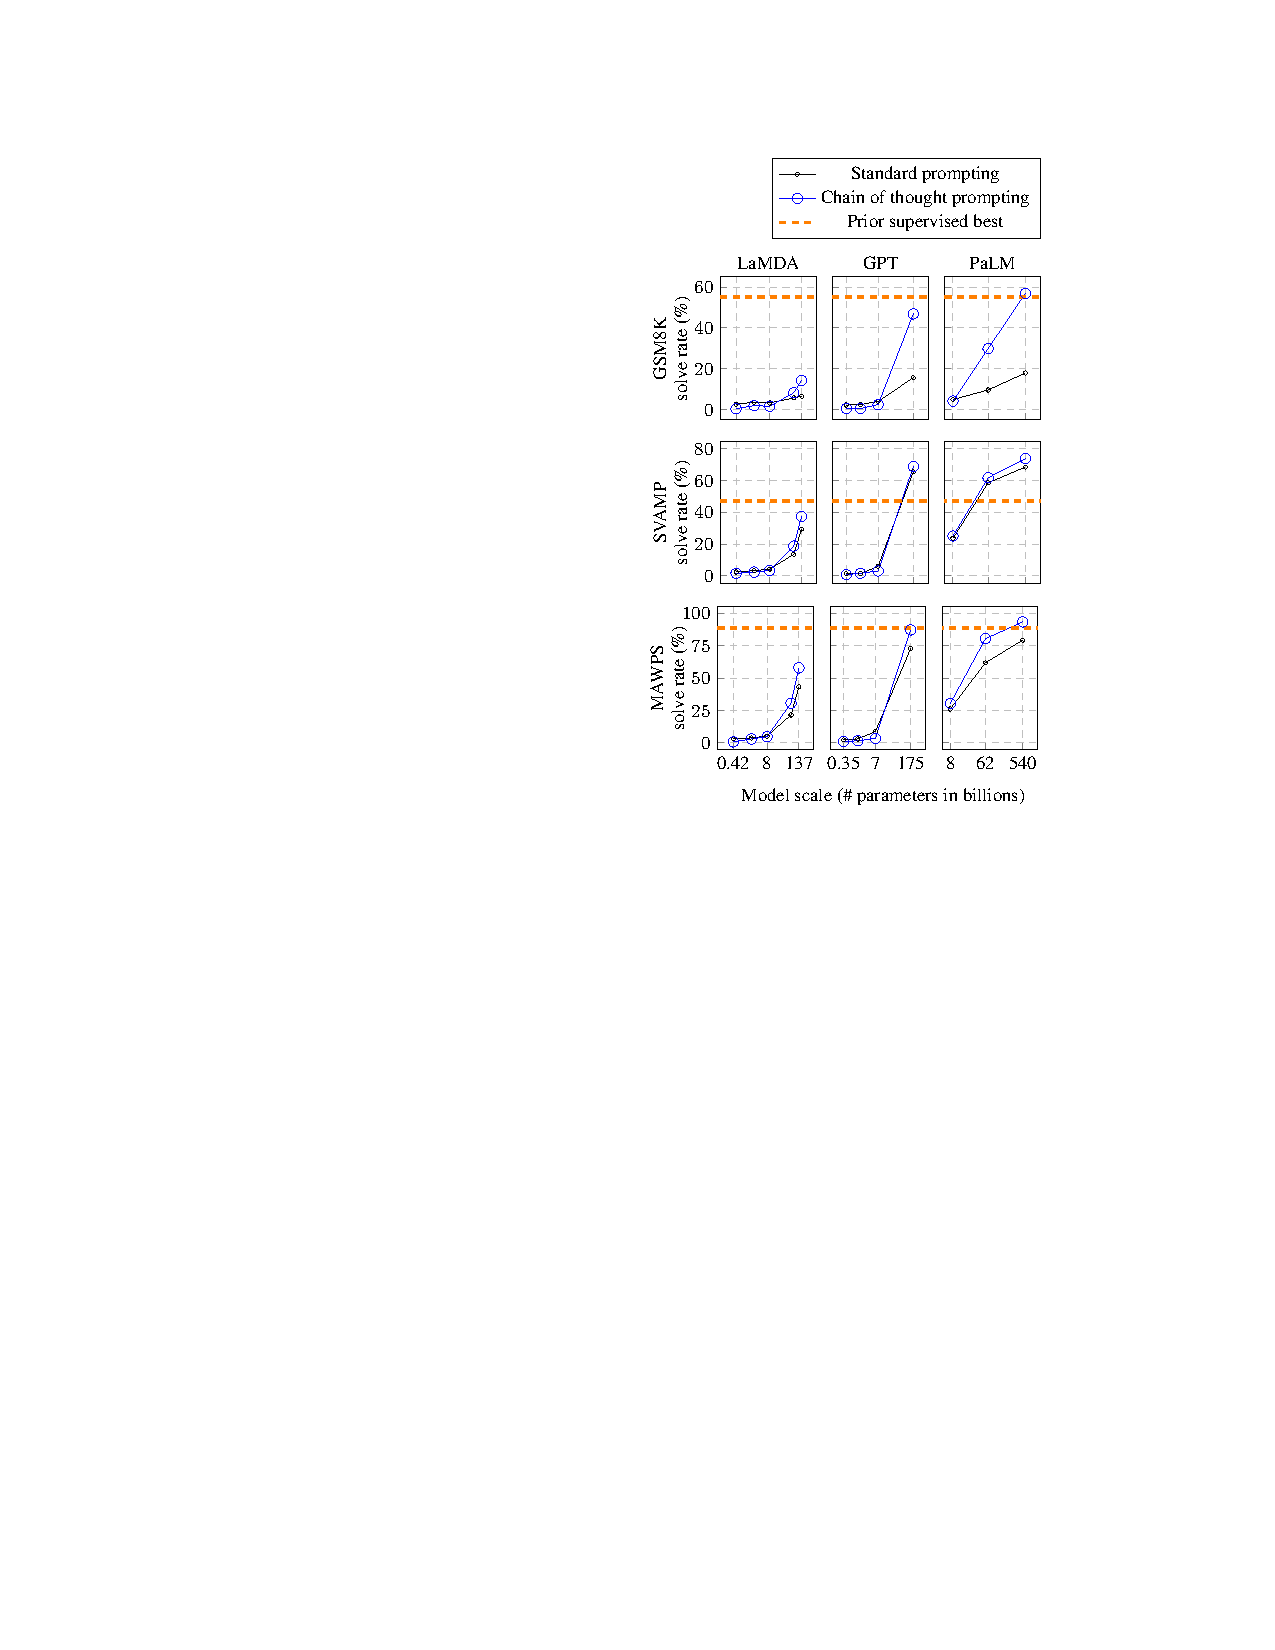
\includegraphics[width=0.4\textwidth,trim={0 9.6cm 0 0cm},clip]{figures/prompting_and_zero_shot/cot_results.pdf}
%   \caption{Performance of three large LMs on three different math world problem datasets. Taken from \citet{wei2022chain}.}
%   \label{fig:cot_result}
% \end{figure}

Chain-of-thought prompting has been shown to significantly improve the ability of large language models to perform complex reasoning. In particular, experiments on a variety of tasks have shown that the ability to generate chains of reasoning is a \textit{emergent} property of model size. This means that larger models are better at generating step-by-step chains of reasoning than smaller models. This has allowed the chain of thought prompting to become the de facto method for querying modern LLMs. 

% This phenomenon is noticeable in the scores reported in \Cref{fig:cot_result}. The results display a significant discrepancy between the solve rate obtained with the chain of thought and with standard prompting on the GSM8k dataset \citep{cobbe2021training} of high school math word problems.

% However, this difference in performance does not seems to be as large for SVAMP and MAWPS. This is because GSM8k consists of complex problems that require multiple reasoning steps, while the other two datasets are made up of simpler problems that, for the most part, only require the application of a single mathematical operator to obtain the final result. This highlights how CoT prompting is most effective in eliciting in-context learning on multi-step reasoning problems.

\subsection{Least to Most Prompting (Problem Decomposition)}

Chain-of-thought prompting has shown impressive results on a variety of natural language reasoning tasks. However, its effectiveness decreases when a given task is more challenging than the examples provided in the prompts. To address this issue, problem decomposition has been proposed both for training \citep{shridhar-etal-2022-automatic} and as a prompting strategy \citep{zhou2023leasttomost}. In this method, a complex problem is broken down into smaller, more manageable sub-problems that are tackled one at a time. The solution to each subproblem helps to solve the next, allowing for a sequential problem-solving process. An example of this prompting technique, often referred to as Least to Most prompting, is provided in \autoref{fig:ltm}. %To decrease the number of prompts, self-ask \citep{press-etal-2023-measuring} proposes an extension to this method and prompts the model to keep asking whether additional follow-up questions are needed.

\begin{figure}[htbp]
    \centering
    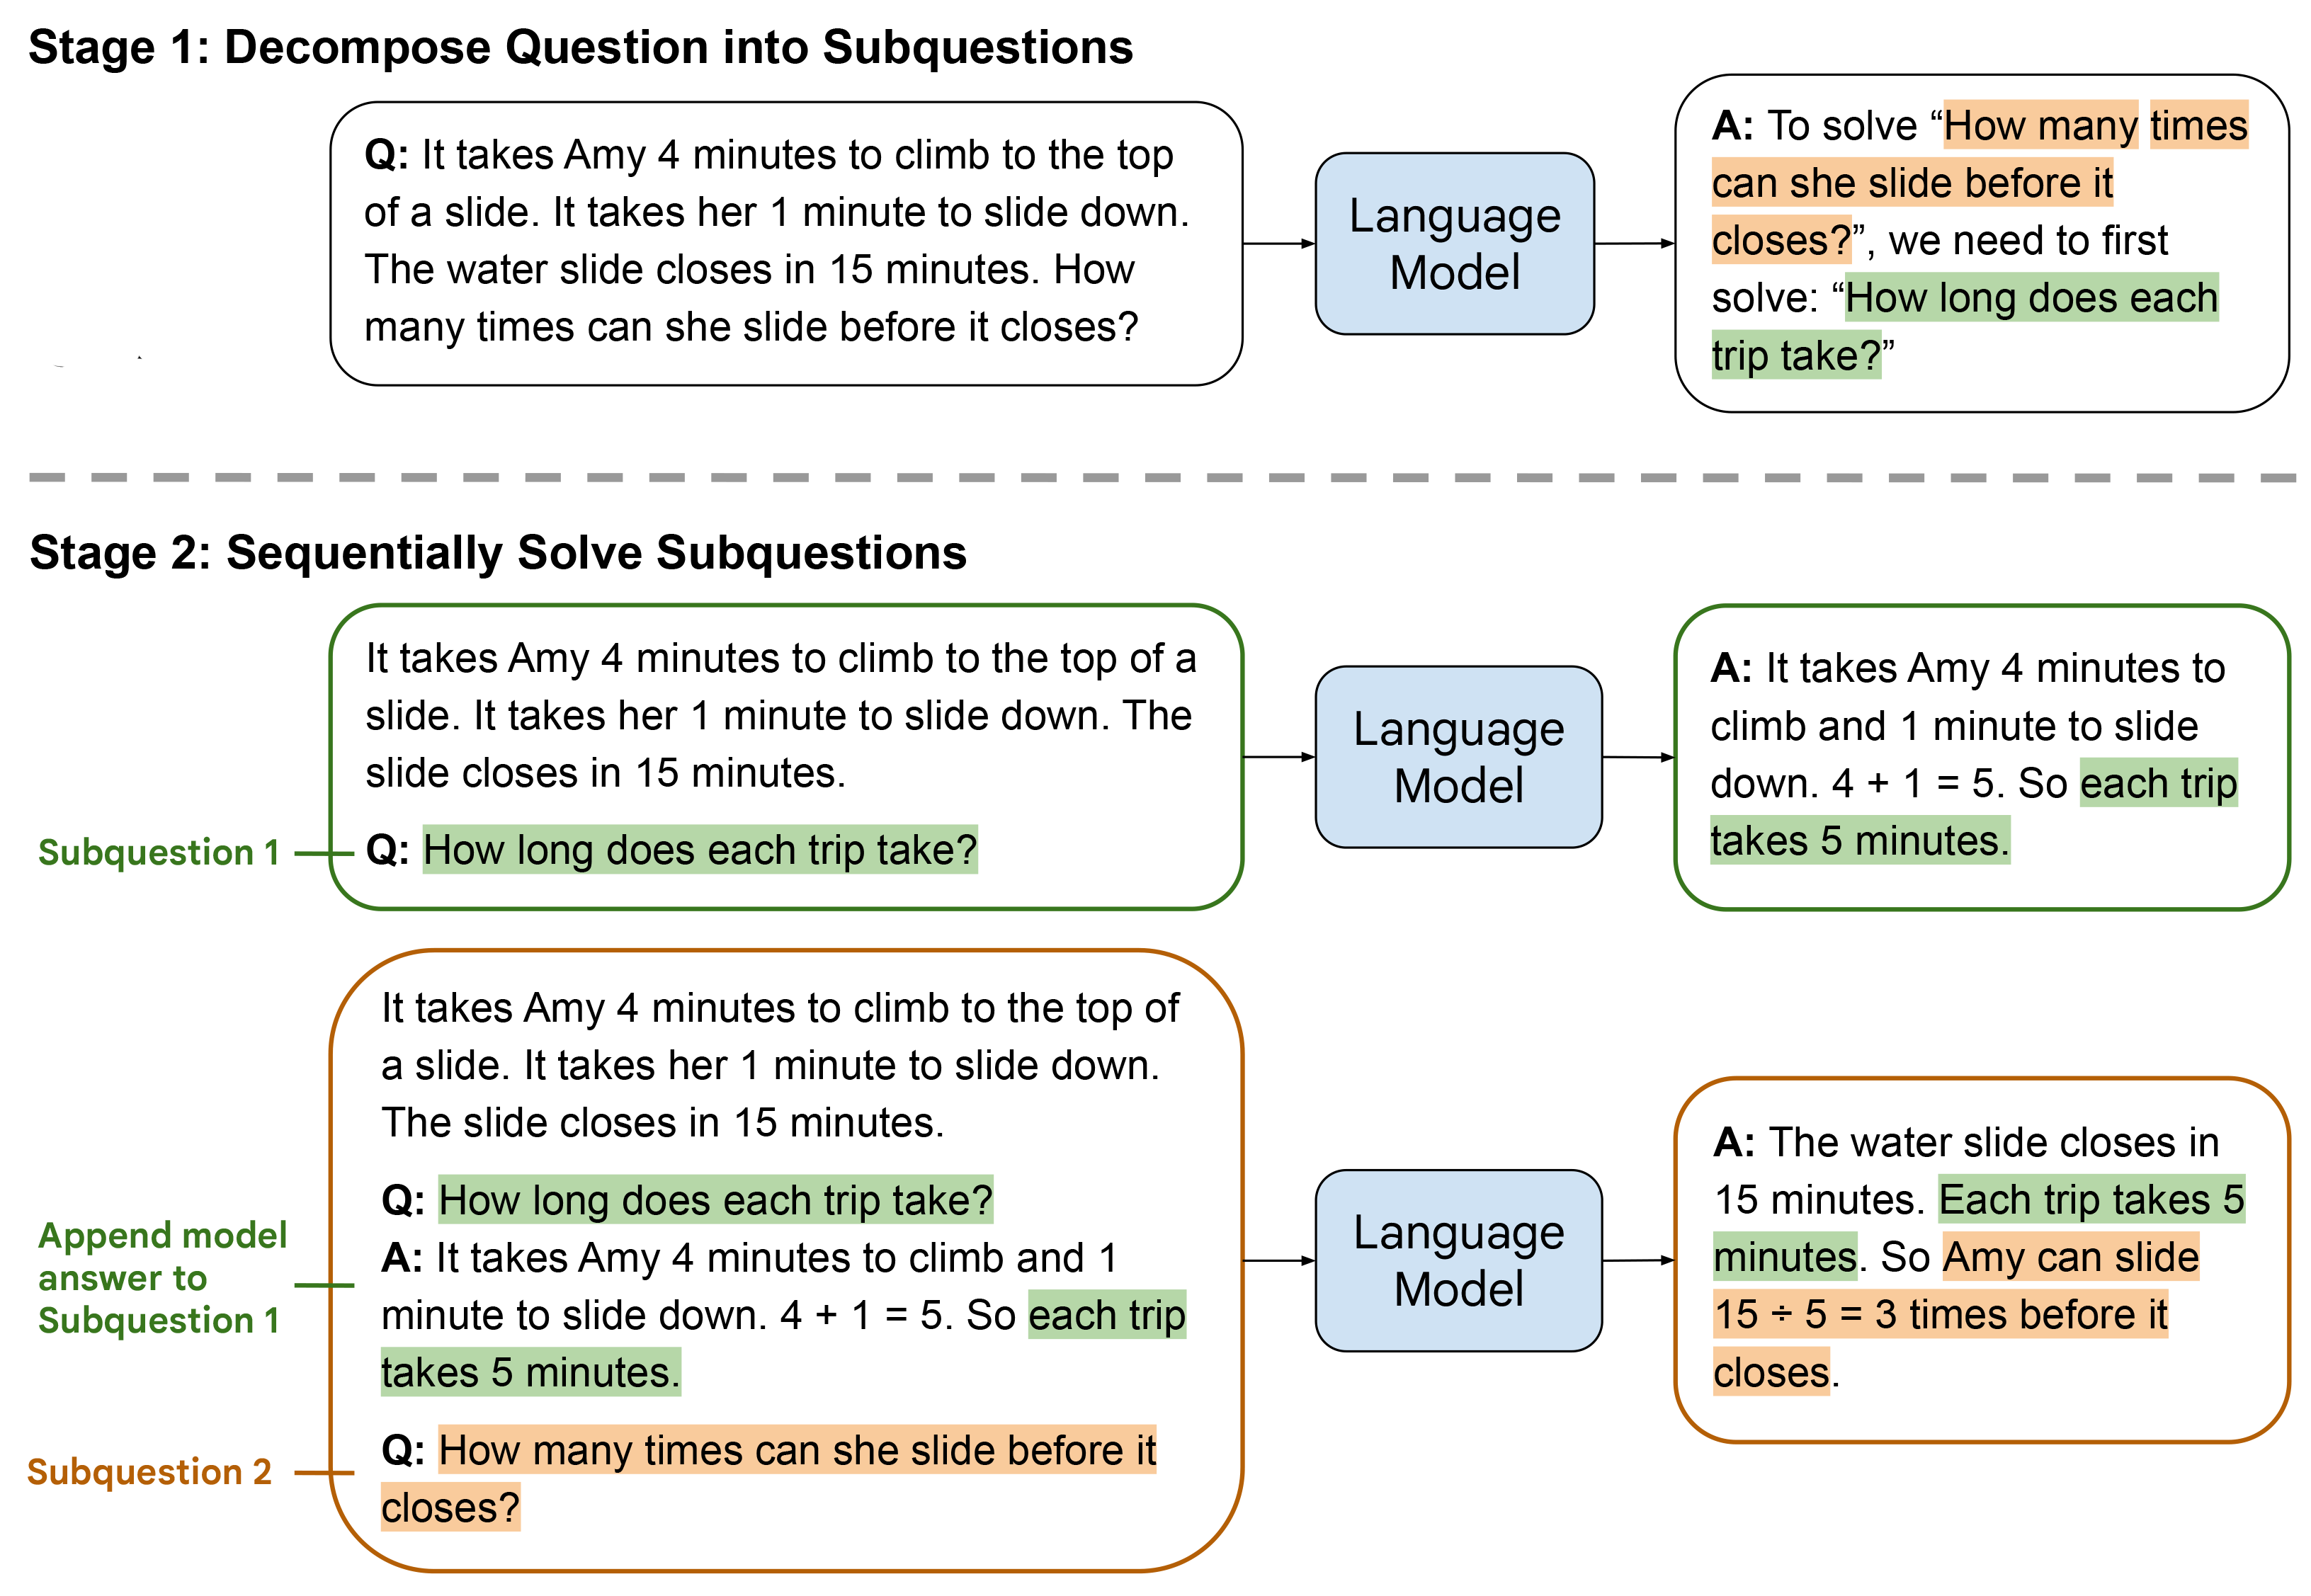
\includegraphics[width=0.9\textwidth]{figures/prompting_and_zero_shot/ltm-pull-fig_new.png}
    \caption{Example of the Least to Most prompting. Subquestions are solved sequentially one by one each in a separate prompt. Taken from \citet{zhou2023leasttomost}.}
    \label{fig:ltm}
\end{figure}

\subsection{Program of Thought Prompting (Structural Thought)}

Approaches like Chain of Thought or Least to Most prompting often struggle with tasks that involve lots of numerical computations as the language model not only needs to generate
the mathematical expressions but also needs to perform the computation in each step. Language models face significant challenges in accurately solving mathematical expressions due to several limitations: Firstly, they frequently make errors in arithmetic calculations, particularly with large numbers. Secondly, they struggle with solving complex mathematical expressions, including polynomial equations and differential equations. Lastly, they are notably inefficient in handling iterative processes, especially when the iterations involve a large number of steps.

To address these challenges and the fact that LLMs are better at producing code than doing math, the concept of program-of-thoughts (PoT) prompting was introduced by \citet{pot}. They propose a method where computational steps are outsourced to an external language interpreter. In the PoT approach, language models are capable of formulating reasoning steps as Python programs. The execution of these programs, and thus the computation, is then carried out by a Python interpreter, enabling more accurate and complex mathematical problem-solving capabilities. A comparison with the chain of thought and PoT is presented in \autoref{fig:pot}.

\begin{figure}[htbp]
    \centering
    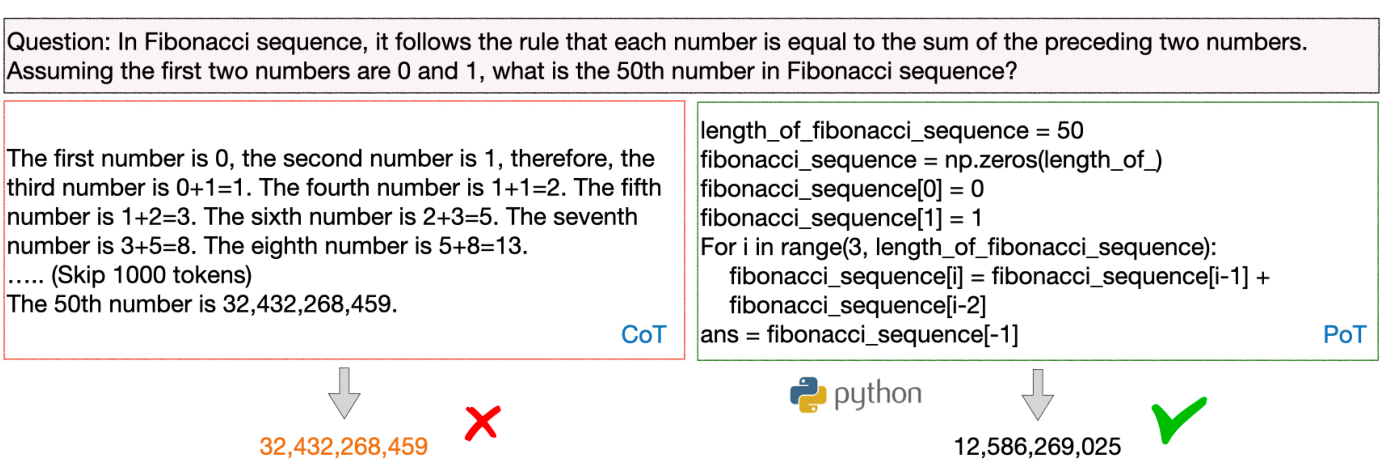
\includegraphics[width=0.9\textwidth]{figures/prompting_and_zero_shot/pot.pdf}
    \caption{Example of the Program of Thought prompting. Taken from \citet{pot}.}
    \label{fig:pot}
\end{figure}

%An extension of the Program of Thought approach is \emph{Faithful Chain of Thought}, or \emph{Faithful CoT}, which is a framework that reasoning into \emph{Translation} and \emph{Problem Solving} phases. The \emph{Translation} phase translates a query (often in natural language format) into a reasoning chain (which uses a lot of symbolic language), and the \emph{Problem Solving} phase where an external solver executes the reasoning chain to derive the answer. The reasoning chain interleaves user-understandable natural language comments and executable symbolic language programs, thus providing faithful interpretability of how the model arrives at the answer. 
A summary of different prompting strategies for solving a math word problem is summarized in \autoref{fig:cc}.

\begin{figure}[htbp]
    \centering
    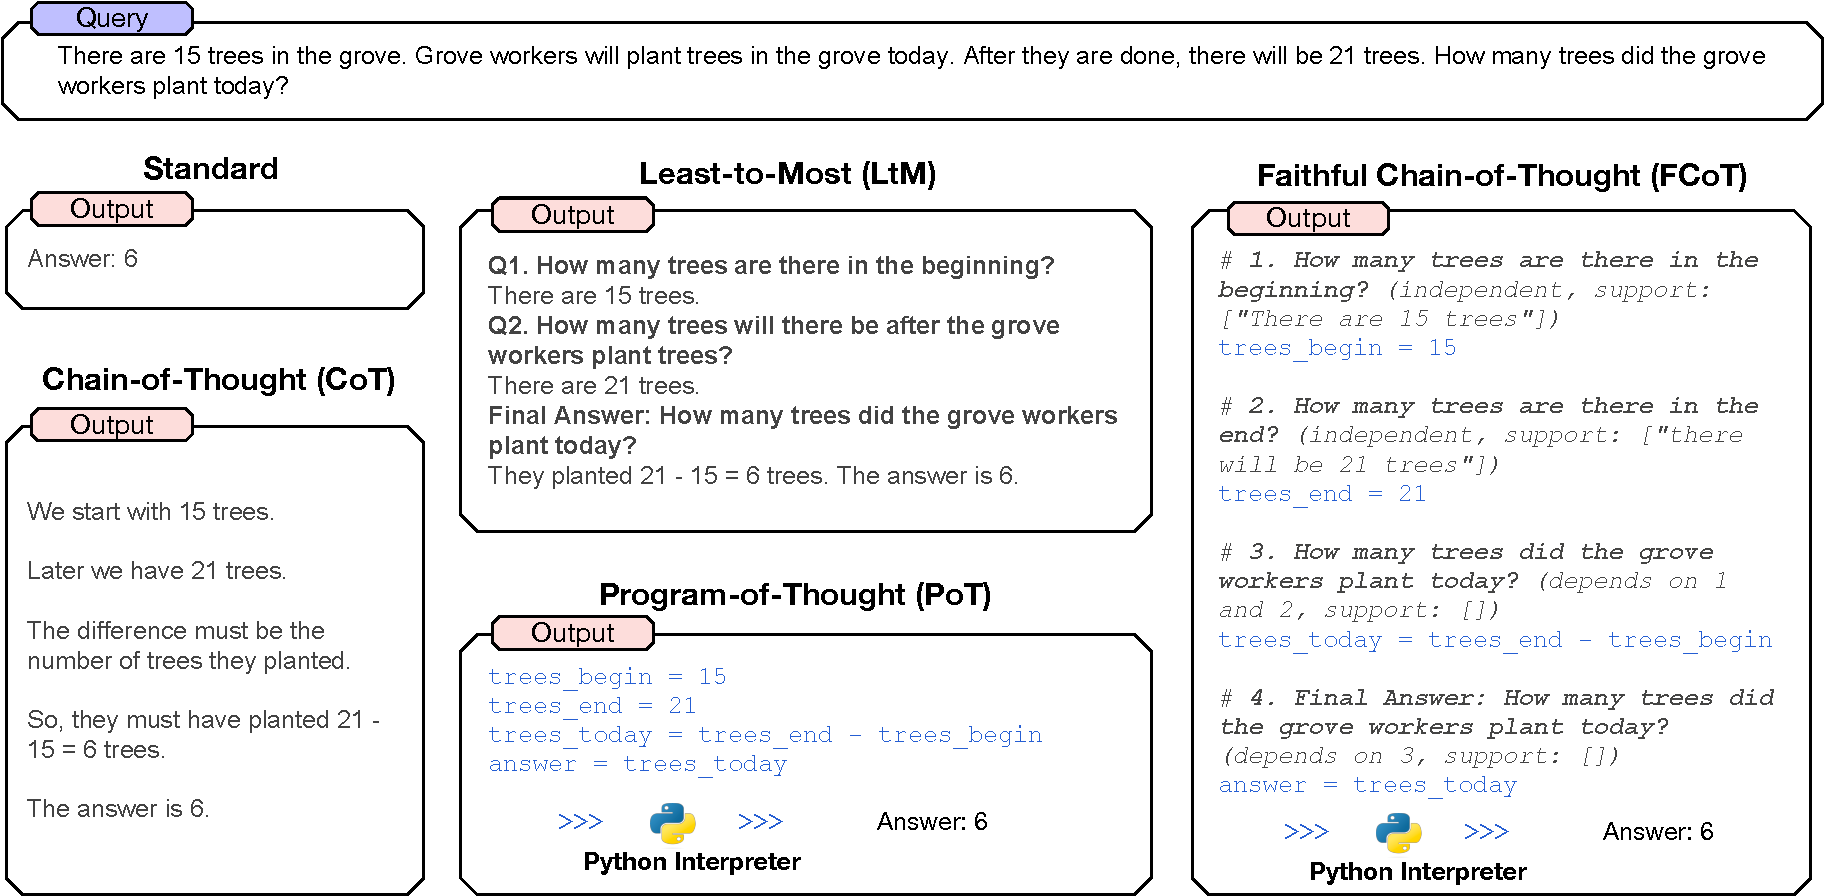
\includegraphics[width=0.9\textwidth]{figures/prompting_and_zero_shot/prompting_strategies.pdf}
    \caption{Example demonstrating different prompting strategies for a given Math Word Problem. Taken from \citet{calibrating-consistency}.}.
    \label{fig:cc}
\end{figure}


\subsection{Performance comparison of different prompting strategies}

It is difficult to conclude whether one prompting strategy is better than the other for a given task because each one is designed for specific types of task. \citet{calibrating-consistency} conducted a study comparing all of the above strategies across nine reasoning datasets, using various open-source and closed models. An average result across all tasks is presented in the \autoref{table:accuracy}. Chain of Thought and Faithful Chain of Thought prompting strategies seem to perform best in most cases, closely followed by Least to Most (LtM) and Program of Thought (PoT). All four of these prompting strategies involve an explanation of intermediate steps, whereas standard prompting directly predicts the answer. In short, \emph{prompting strategies that involve intermediate steps perform better than a direct prediction of the answer}.

\begin{table}[h]
    \centering
    \begin{tabular}{l c c c c c}
    \toprule

        \textbf{Model} & \textbf{Standard} & \textbf{CoT} & \textbf{LtM} & \textbf{PoT}  & \textbf{FCoT}\\ 
        \midrule
         Codex & 57.1 &	81.3 & 74.3 &	80.0 &	\textbf{83.4} \\ 
         GPT-3.5.turbo & 64.9&	\textbf{77.6} &	\textbf{77.6} &	72.5 &	76.8\\ 
         GPT-4 & 79.3	&88.3	&87.3	&84.4	&\textbf{90.9}\\ 
         LLaMA-7B & 40.1	&\textbf{56.4}	&46.0	&47.4	&50.2\\
         LLaMA-13B&43.2	&\textbf{66.8}	&58.2	&56.9	&62.2\\
         LLaMA-70B& 58.0	&\textbf{82.0}	&73.3	&73.6	&77.0\\
         Mistral-7B& 49.9	&\textbf{73.5}	&61.9	&66.5	&71.2\\
         Mistral-7B-instruct & 43.7	&63.6	&56.0	&60.0	&\textbf{67.1}\\
        \bottomrule
    \end{tabular}
    \vspace{-0.03in}
    \caption{Accuracy (in \%) averaged across all datasets for various LLMs. The best accuracy for a given model is highlighted in \textbf{bold}. Table taken from \citet{calibrating-consistency}.}
    \label{table:accuracy}
\end{table}

\subsection{Self-consistency}

Greedy decoding (setting with temperature $T=0$) can be considered the most naive decoding strategy, where an LM is given a prompt with or without in-context examples and an output is generated. However, this limits the creativity of the LM by generating only one greedy sample per input. An extension to the decoding strategy called \emph{self-consistency} \citep{selfconsistency} provides an alternative to simple greedy decoding by generating a variety of outputs (with $T>0$) instead of just following the most likely one. 
%The method introduces a latent variable $r_i$, a sequence of tokens representing $i$-th reasoning path and is used to parse the final answer $a_i$. 
Taking an example of the task of solving reasoning problems, the most consistent answer is defined by sampling $n$ candidate pairs of reasoning paths and their corresponding final numerical answer $(r_i, a_i)$ and marginalizing over $r_i$ by taking a majority vote over $a_i$: 
\begin{align}
    \arg\max_{a} \sum_{i=1}^{n} \mathbbm{1}(a_i = a).
\end{align}
The same idea could be used for other tasks by taking the most consistent answer over the range of sampled outputs. The \emph{self-consistency} approach argues that a task, say a reasoning task, often allows for several different lines of thought that converge on the same correct solution. 
In this case, the most frequently generated solution is more likely to be the correct one.
A comparison with a single chain of thought strategy is demonstrated in \autoref{fig:self-con}.

\begin{figure}[ht]
    \centering
    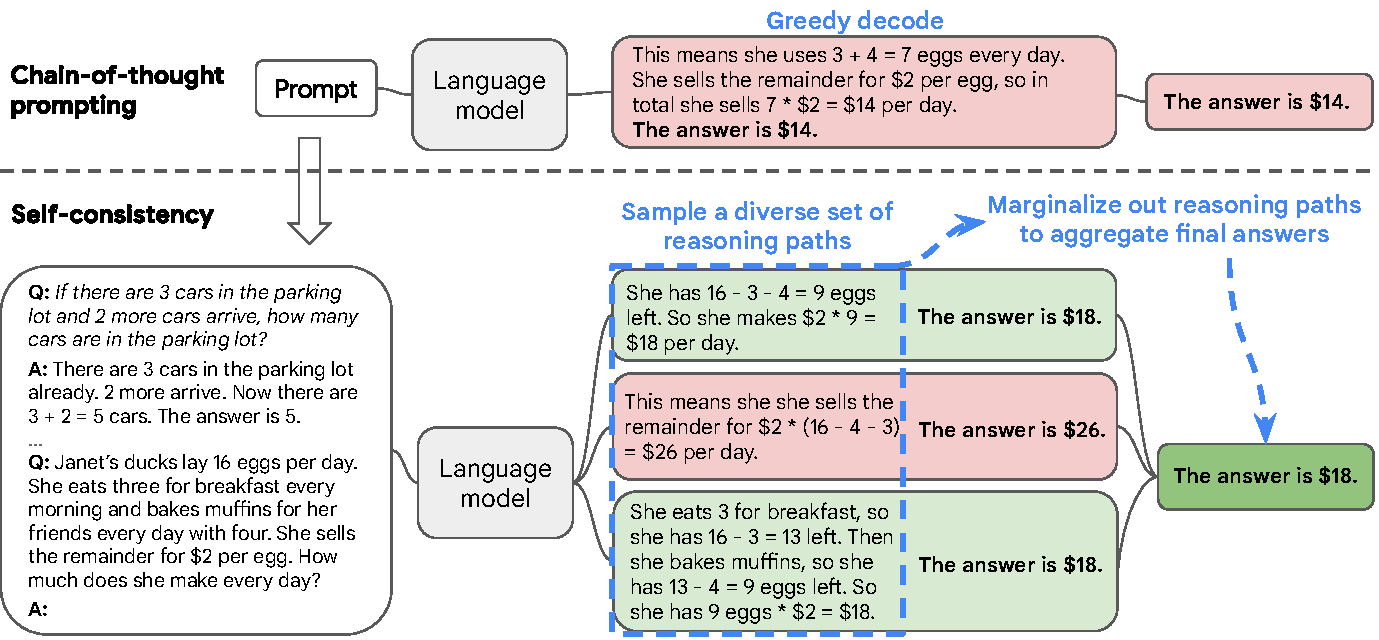
\includegraphics[width=0.8\textwidth]{figures/prompting_and_zero_shot/self_consistency_fig.pdf}
    \caption{Comparison of the Chain of Thought with and without self-consistency decoding. In this example, $n=3$ reasoning paths are sampled from the model and the most frequent answer is taken as the final answer. Take from \citet{selfconsistency}.
    }
    \label{fig:self-con}
\end{figure}